Troopers may use vehicles, such as motorcycles and hoverbikes, for enhanced mobility.

\paragraph*{Vehicle Card}

The unit card shows the current capabilities of a vehicle and tracks damage.
A unit card can be formatted in any way so long as it contains all the essential information.
Below is a sample unit card for a basic vehicle.

\begin{figure}[H]
  \centering
  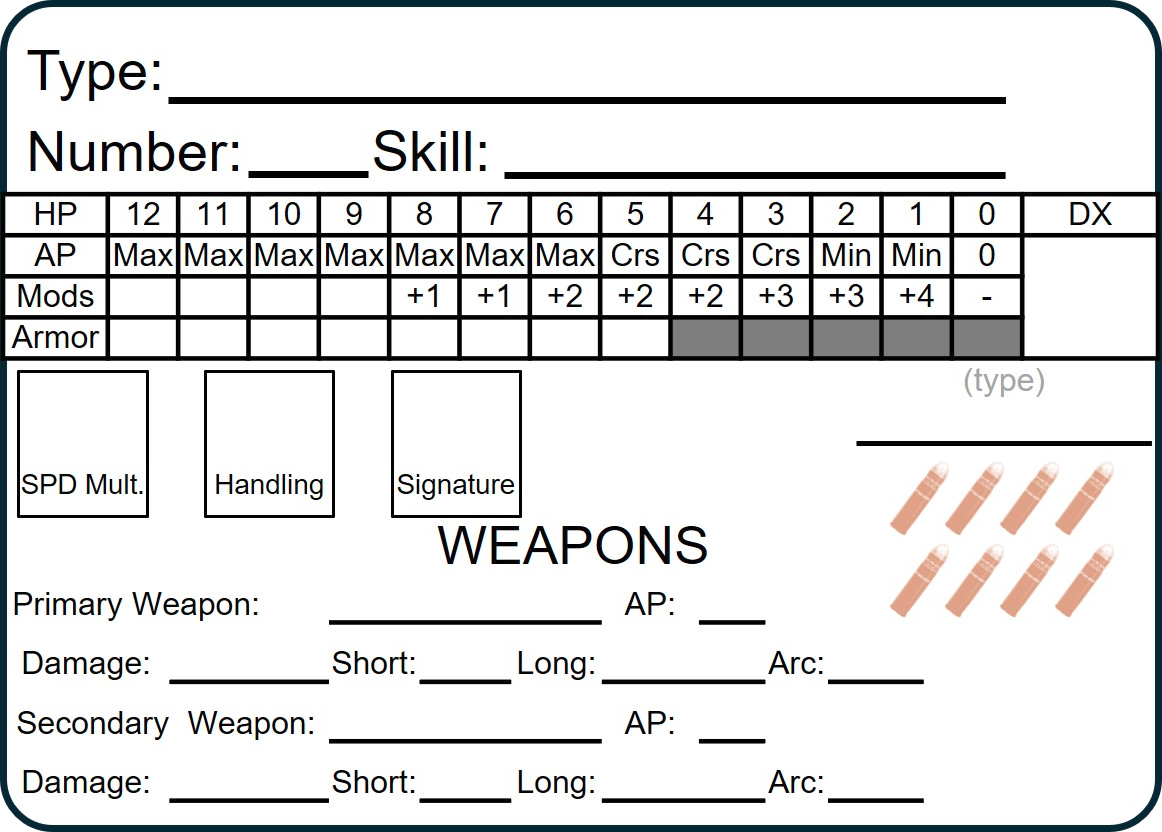
\includegraphics[alt='Sample Vehicle', width=5.63in, height=4in]{img/Vehicle.png}
  \caption*{Basic Vehicle Unit Card}
\end{figure}

Basic information about the vehicle, such as its type and id number.

Damage to the vehicle is tracked in the HP section.
HP cells are labeled by their HP value, from highest to lowest, 12 to 0, from left to right.
HP cells are fully crossed out when the vehicle takes standard damage (X).
Vehicles ignore bludgeoning damage (\textbackslash).
The current HP of the vehicle is given by the first cell to the right of the lowest fully marked HP cell.

The maximum valid movement mode for the vehicle is given in the AP section.
Use the value in the column corresponding to the vehicle's current HP.
For example, if the vehicle has 5 HP, then it can only use the minimum or cruse movement modes.

Similarly, the modifier section tracks the current modifier for the vehicle's target numbers based upon current HP.
This modifier only applies to vehicle control checks and attacks made with weapons mounted to the vehicle.
For example, if the vehicle has 5 HP, then add +2 to all target numbers.

If the vehicle's armor value is given by in the armor section.
Lethal damage (X) destroys armor before damaging HP cells.
If a single attack does more damage than the remaining armor, first mark all remaining armor and then roll 2D6 to determine where to apply the remaining damage.
The standard armor of a scout vehicle is 4 and the standard armor of an assault vehicle is 8.

The vehicle's speed multiplier is given by the speed multiplier section.
This is how many dots the bike moves for each AP spend on movement.
The standard speed of a scout vehicle is 3 and the standard speed of an assault vehicle is 2.

The vehicle's handling modifier is given by the handling section.
This modifier applies to all control checks.
The standard handling modifier of a scout vehicle is +0 and the standard handling modifier of an assault vehicle is +1.

The signature section gives any modifiers for attacks on the vehicle.
Larger vehicles are easier to hit.
The signature modifier of a scout vehicle is -1 and the standard signature modifier of an assault vehicle is -2.

The ammo section lists any additional ammo for any weapons mounted on the vehicle.

The weapons section list the weapons mounted on the vehicle, along with their orientation, damage values, and range brackets.
The standard scout vehicle has no weapons and the standard assault vehicle has two forward mounted weapons.
Light machine guns, from the crew served weapons table, are the most weapons mounted on vehicles.

\paragraph*{Map Template}

The map template shows the location of the vehicle on the map.
Below is a sample map template for a basic vehicle.

\begin{figure}[H]
  \centering
  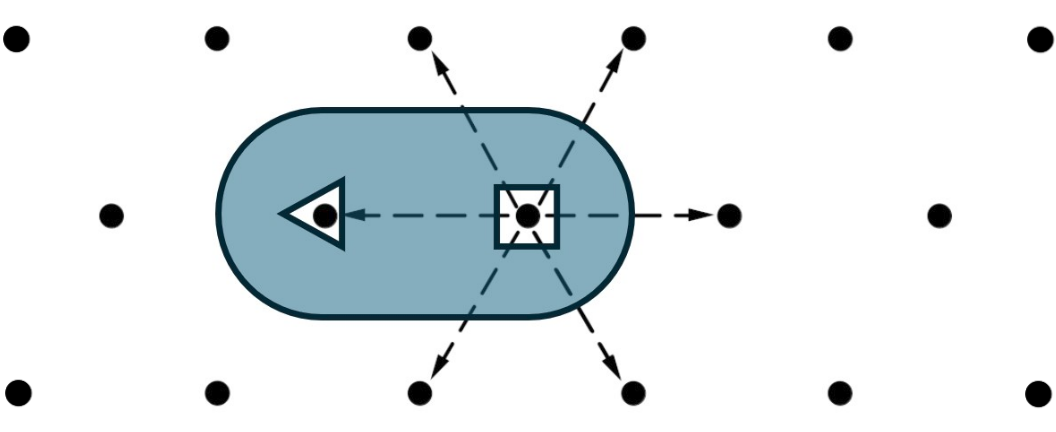
\includegraphics[alt='Sample Vehicle Map Template', width=6.5in, height=3.66in]{img/MapVehicle.png}
  \caption*{Basic Vehicle Map Template}
\end{figure}

Motorcycles and hoverbikes occupy two dots on the map.
On the given template, the triangle indicates the front of the vehicle and the square indicates rear of the vehicle.

The trooper sits on the rear dot of the template, and weapon attacks to or from the trooper are measured from this point.
Weapon attacks from the vehicle are also measured from the rear dot of the template, but weapon attacks to the vehicle may target either dot.

\paragraph*{Movement}

In order to use a vehicle, a trooper must first mount the vehicle and turn it on.
The vehicle stays on until turned off.

\begin{table}[H]
\ifthenelse{\not \equal{\outworldsMode}{mode-web}}{\fontfamily{Montserrat-LF}}{\small}\selectfont
\centering
\newcolumntype{R}[1]{>{\raggedleft\let\newline\\\arraybackslash\hspace{0pt}}m{#1}}
\begin{tabular}{!{\Vline{1pt}} m{9em} !{\Vline{1pt}} R{4.5em} !{\Vline{1pt}}}
\Hline{1pt}
\rowcolor{black!30}  \bfseries{Action} & \bfseries{AP Cost} \\
\Hline{1pt}
Mount/Dismount & 2  \\
Turn on/off    & 1  \\
\Hline{1pt}
\end{tabular}
\caption*{Vehicle AP Costs}
\end{table}

Once a trooper is on the vehicle, they must select a movement mode for the turn.
A trooper can only select a movement mode if they have sufficient remaining AP for that movement mode and the vehicle currently supports that movement mode.
The trooper must spend the amount of AP corresponding to the selected movement mode. For example, if the cruse movement mode is selected, the trooper must spend 2-4 AP on movement, including accelerating, decelerating, movement, and turning.
No more than 8 total AP may be spent on vehicle and trooper movement in a turn.

If the trooper or bike cannot finish spending sufficient AP for the selected movement mode due to damage taken during movement, the vehicle automatically wipes out.

\begin{table}[H]
\ifthenelse{\not \equal{\outworldsMode}{mode-web}}{\fontfamily{Montserrat-LF}}{\small}\selectfont
\centering
\newcolumntype{R}[1]{>{\raggedleft\let\newline\\\arraybackslash\hspace{0pt}}m{#1}}
\begin{tabular}{!{\Vline{1pt}} m{10em} !{\Vline{1pt}} R{4.5em} !{\Vline{1pt}}}
\Hline{1pt}
\rowcolor{black!30}  \bfseries{Movement Mode} & \bfseries{AP Used} \\
\Hline{1pt}
Minimum &   1  \\
Cruise  & 2-4  \\
Max     & 5-8  \\
\Hline{1pt}
\end{tabular}
\caption*{Vehicle Movement Modes}
\end{table}

Accelerating from a full stop costs 1 AP and decelerating to a full stop costs 2 AP.
The speed modifier on the vehicle card states how many dots the vehicle moves for each AP spent to move.
The vehicle also moves this number of dots while starting from a full stop or slowing to a full stop.
The vehicle cannot pass through impassible obstacles or solid obstructions.

\begin{table}[H]
\ifthenelse{\not \equal{\outworldsMode}{mode-web}}{\fontfamily{Montserrat-LF}}{\small}\selectfont
\centering
\newcolumntype{R}[1]{>{\raggedleft\let\newline\\\arraybackslash\hspace{0pt}}m{#1}}
\begin{tabular}{!{\Vline{1pt}} m{10em} !{\Vline{1pt}} R{4.5em} !{\Vline{1pt}}}
\Hline{1pt}
\rowcolor{black!30}  \bfseries{Action} & \bfseries{AP Cost} \\
\Hline{1pt}
Start from full stop & 1  \\
Slow to full stop    & 2  \\
Move                 & 1  \\
\Hline{1pt}
\end{tabular}
\caption*{Vehicle Movement AP Costs}
\end{table}

While moving, the vehicle may spend AP to turn.
A vehicle must move forward by at least 1 dot before turning, and turns can be executed at any point during the vehicle's movement.
The front of the vehicle stays in place during a turn while the rear of the vehicle swings to a new dot.
Since a 60 degree (1 dot) turn costs no AP to execute, it is the only turn that can be executed during the minimum movement mode.

\begin{table}[H]
\ifthenelse{\not \equal{\outworldsMode}{mode-web}}{\fontfamily{Montserrat-LF}}{\small}\selectfont
\centering
\newcolumntype{R}[1]{>{\raggedleft\let\newline\\\arraybackslash\hspace{0pt}}m{#1}}
\begin{tabular}{!{\Vline{1pt}} m{8em} !{\Vline{1pt}} R{4.5em} !{\Vline{1pt}}}
\Hline{1pt}
\rowcolor{black!30}  \bfseries{Action} & \bfseries{AP Cost} \\
\Hline{1pt}
 60 degree turn & 0  \\
120 degree turn & 1  \\
180 degree turn & 2  \\
\Hline{1pt}
\end{tabular}
\caption*{Vehicle Turning Movement AP Costs}
\end{table}

When executing a 120 or 180 degree turn, the trooper must make a control check.
A control check is a 2D6 check with the target number gives by the chart below.
Apply all modifiers for damage to the trooper and the vehicle.
If the control check fails, the vehicle wipes out.

\begin{table}[H]
\ifthenelse{\not \equal{\outworldsMode}{mode-web}}{\fontfamily{Montserrat-LF}}{\small}\selectfont
\centering
\newcolumntype{R}[1]{>{\raggedleft\let\newline\\\arraybackslash\hspace{0pt}}m{#1}}
\begin{tabular}{!{\Vline{1pt}} m{8em} !{\Vline{1pt}} R{8em} !{\Vline{1pt}}}
\Hline{1pt}
\rowcolor{black!30}  \bfseries{Action} & \bfseries{Target Number} \\
\Hline{1pt}
 60 degree turn & --  \\
120 degree turn &  6  \\
180 degree turn &  9  \\
\Hline{1pt}
\end{tabular}
\caption*{Vehicle Turning Control Check}
\end{table}

Decelerating to a full stop while using the cruise or maximum movement modes also requires a control check.
A trooper may incorporate a turn into the deceleration to a full stop, but this increases the difficulty of the control check.

\begin{table}[H]
\ifthenelse{\not \equal{\outworldsMode}{mode-web}}{\fontfamily{Montserrat-LF}}{\small}\selectfont
\centering
\newcolumntype{R}[1]{>{\raggedleft\let\newline\\\arraybackslash\hspace{0pt}}m{#1}}
\begin{tabular}{!{\Vline{1pt}} m{8em} !{\Vline{1pt}} R{8em} !{\Vline{1pt}}}
\Hline{1pt}
\rowcolor{black!30}  \bfseries{Action} & \bfseries{Target Number} \\
\Hline{1pt}
 no turn        & 4  \\
 60 degree turn & 4  \\
120 degree turn & 6  \\
180 degree turn & 8  \\
\Hline{1pt}
\end{tabular}
\caption*{Vehicle Breaking Control Check}
\end{table}

If vehicle activates in or moves into a firing arc, the firing unit may choose to fire as long as the firing trooper has line of sight.
For each AP spent on movement, the vehicle must start or end that segment of movement in the firing unit's firing arc to be a valid target.
For example, if a vehicle has a speed modifier of 3 and is only in the firing unit's firing arc on the second dot for a set of 3 dots of movement, then the firing unit cannot fire on the vehicle.

The firing unit may target either the vehicle or the trooper, but not both.
The firing unit must have a valid line of sight to the rear dot of the vehicle to target the trooper on the vehicle.
The vehicle and trooper together can only be attacked once for each AP spent on movement.
For example, if a vehicle has a speed modifier of 2, then the vehicle and trooper together can only be attacked once for each set of 2 dots traversed.

If the damage to the vehicle makes the current movement mode invalid or damage to the trooper leaves insufficient AP to complete the current movement mode, then the vehicle automatically wipes out as if it had failed a control check.

Explosive damage is applied to both the vehicle and trooper.
Use the closest point on the vehicle to the center of the explosion to determine how much damage to apply to the vehicle.
Vehicles are not effected by incendiary damage, but incendiary damage is still applied to the trooper on the vehicle.

\paragraph*{Vehicle Damage}

Vehicles are not effected by bludgeoning damage.
When applying damage to a vehicle, first apply the damage to any remaining armor.
If there is remaining damage after the armor is destroyed, roll 2D6.
This is the initial cell to apply damage in.
Starting with the initial cell, cross out the number of cells given by the remaining damage value, skipping any previously crossed out cells.

\paragraph*{Wipe Out}

If a trooper fails a control check, has insufficient AP to complete the current movement mode, or the vehicle is damaged and cannot complete the movement mode, then the vehicle and trooper wipe out.

If the vehicle was attempting to turn, then set the rear of the vehicle as if it had completed a 60 degree shallower turn.
Then move the vehicle in a straight line along the original direction of travel.
If the vehicle was using the cruise movement mode, then it skids the number of dots given by 1 AP of movement, and if the vehicle was using the maximum movement mode, then it skids the number of dots given by 2 AP of movement.
The vehicle is prone once it completes the skid.

For example, if trooper wiped out while executing a 120 degree turn, then set the rear of the vehicle as if it had completed a 60 degree turn.
The vehicle then skids along the ground in a straight line from this point.
If the vehicle was using the maximum movement mode and moves 3 dots per each AP spent on movement, then the vehicle skids 6 dots.

\begin{table}[H]
\ifthenelse{\not \equal{\outworldsMode}{mode-web}}{\fontfamily{Montserrat-LF}}{\small}\selectfont
\centering
\newcolumntype{R}[1]{>{\raggedleft\let\newline\\\arraybackslash\hspace{0pt}}m{#1}}
\begin{tabular}{!{\Vline{1pt}} m{10em} !{\Vline{1pt}} R{4.5em} !{\Vline{1pt}}}
\Hline{1pt}
\rowcolor{black!30}  \bfseries{Movement Mode} & \bfseries{Damage} \\
\Hline{1pt}
Minimum & 0  \\
Cruise  & 1  \\
Max     & 2  \\
\Hline{1pt}
\end{tabular}
\caption*{Vehicle Wipe Out Damage}
\end{table}

If the vehicle hits an impassible obstacle or solid obstruction while skidding, then stop the skid immediately and apply ramming damage to the vehicle and trooper.
If the vehicle does not hit an impassible obstacle or solid obstruction, then after the skid is completed apply wipe out damage to the vehicle and trooper.

After wiping out, it costs 3 AP for a trooper to climb out from underneath a vehicle and and additional 3 AP to lift the vehicle to an upright position.
The trooper may chose to be prone or standing after climbing out from underneath the vehicle but remains in the same dot.
A trooper must be standing to lift the vehicle to an upright position.

\begin{table}[H]
\ifthenelse{\not \equal{\outworldsMode}{mode-web}}{\fontfamily{Montserrat-LF}}{\small}\selectfont
\centering
\newcolumntype{R}[1]{>{\raggedleft\let\newline\\\arraybackslash\hspace{0pt}}m{#1}}
\begin{tabular}{!{\Vline{1pt}} m{8em} !{\Vline{1pt}} R{4.5em} !{\Vline{1pt}}}
\Hline{1pt}
\rowcolor{black!30}  \bfseries{Action} & \bfseries{AP Cost} \\
\Hline{1pt}
Crawl out    & 3  \\
Lift vehicle & 3  \\
\Hline{1pt}
\end{tabular}
\caption*{Vehicle Wipe Out Costs}
\end{table}

\paragraph*{Combat}

A trooper may make four types of attacks while on a vehicle - ramming, melee, movement fire, and standard fire.
All of these attacks, except standard fire, occur during the movement of the vehicle.

When a vehicle's front dot is in a dot adjacent to an enemy unit, the vehicle may make a ramming attack.
A trooper on a vehicle cannot be targeted by a ramming attack; only the vehicle may be targeted.

First, apply the ramming damage to the targeted unit.
Only apply the ramming damage to the vehicle executing the ramming attack if it has no remaining armor.
Then make a control check with a base target number of 6.
Apply all modifiers for damage to the trooper and the vehicle.
On a failed control check, the vehicle wipes out, as above.

\begin{table}[H]
\ifthenelse{\not \equal{\outworldsMode}{mode-web}}{\fontfamily{Montserrat-LF}}{\small}\selectfont
\centering
\newcolumntype{R}[1]{>{\raggedleft\let\newline\\\arraybackslash\hspace{0pt}}m{#1}}
\begin{tabular}{!{\Vline{1pt}} m{10em} !{\Vline{1pt}} R{4.5em} !{\Vline{1pt}}}
\Hline{1pt}
\rowcolor{black!30}  \bfseries{Movement Mode} & \bfseries{Damage} \\
\Hline{1pt}
Minimum & 1X  \\
Cruise  & 3X  \\
Max     & 5X  \\
\Hline{1pt}
\end{tabular}
\caption*{Vehicle Ramming Damage}
\end{table}

When a vehicle's rear dot is adjacent to enemy unit, the trooper on the vehicle may make a melee attack as long as a melee weapon is the trooper's current active weapon.
The trooper's active melee weapon does additional lethal damage based upon the movement mode of the vehicle.

First make a melee attack as normal, applying all appropriate modifiers, including a +2 modifier for a movement attack.
On a successful attack, apply the melee damage to the enemy trooper including the additional lethal damage given in the chart below.
After resolving the attack, make a control check with a base target number of 6.
Apply all modifiers for damage to the trooper and the vehicle.
On a failed control check, the trooper wipes out, as above.

\begin{table}[H]
\ifthenelse{\not \equal{\outworldsMode}{mode-web}}{\fontfamily{Montserrat-LF}}{\small}\selectfont
\centering
\newcolumntype{R}[1]{>{\raggedleft\let\newline\\\arraybackslash\hspace{0pt}}m{#1}}
\begin{tabular}{!{\Vline{1pt}} m{10em} !{\Vline{1pt}} R{4.5em} !{\Vline{1pt}}}
\Hline{1pt}
\rowcolor{black!30}  \bfseries{Movement Mode} & \bfseries{Damage} \\
\Hline{1pt}
Minimum & +0X  \\
Cruise  & +1X  \\
Max     & +2X  \\
\Hline{1pt}
\end{tabular}
\caption*{Vehicle Melee Damage}
\end{table}

The trooper on the vehicle may make attacks with the movement fire rules with their current active weapon or any weapons mounted on the vehicle.
A trooper may only use a secondary weapon, SMG, grenade, or satchel charge while on a vehicle.

As with standard movement fire, add a +2 modifier to the target number.
Burst fire weapons may be fired multiple times during movement if the trooper has sufficient AP, and the vehicle may continue moving after firing.
If the trooper is using an explosive weapon, the explosive damage is still resolved after all troopers have moved, as usual.

If a trooper is a passenger in a larger vehicle, such as an assault vehicle, then only apply a +1 modifier for movement fire.
This passenger trooper may use primary weapons to make movement fire attacks.

After movement, the trooper may automatically establish a 2 AP firing arc with any weapons mounted on the vehicle for 0 AP.
